
%(BEGIN_QUESTION)
% Copyright 2008, Tony R. Kuphaldt, released under the Creative Commons Attribution License (v 1.0)
% This means you may do almost anything with this work of mine, so long as you give me proper credit

En av problemene med enkel av/på regulering er at pådragsorganet går av og på ofte. Dette kan skape slitasje og kortere levetid for komponenten. 

En løsning på dette problemet er å lage systemet slik at det har et "gap" eller er "bånd" som de operer innenfor, istedenfor et enkelt settpunkt. I praksis er det to settpunkt: et øvre- og nedresettpunkt. Dette kalles ofte av/på regulering med differensial eller av/på regulering med dødbånd. Her vises en enkel holdekrets for dødbåndsregulering av temperaturen i en ovn. 

$$\includegraphics[width=15.5cm]{i01450x01.eps}$$

I tilfellet med denne ovnen, av/på regulering med dødbånd vil si at varmeelementer ikke vil slå seg på før temperaturen kommer under nedre settpunkt, og det vil ikke slå seg av før temperaturen kommer over øvre settpunkt.

$$\includegraphics[width=15.5cm]{i01450x02.eps}$$

Tegn grafen til ovnens temperatur over tid når reguleringssystmet styrer det. Vis også hvordan grafen til et av/på reguleringsystem uten dødbånd ville sett ut. 

\underbar{file i01450}
%(END_QUESTION)





%(BEGIN_ANSWER)

$$\includegraphics[width=15.5cm]{i01450x03.eps}$$

%(END_ANSWER)





%(BEGIN_NOTES)

The behavior of a differential gap control system is quite a bit ``looser'' than that of a simple (single-point) on-off control, but at least we do not cycle the final control element nearly as often.

\vskip 20pt \vbox{\hrule \hbox{\strut \vrule{} {\bf Virtual Troubleshooting} \vrule} \hrule}

This question is a good candidate for a ``Virtual Troubleshooting'' exercise.  Presenting the diagram to students, you first imagine in your own mind a particular fault in the system.  Then, you present one or more symptoms of that fault (something noticeable by an operator or other user of the system).  Students then propose various diagnostic tests to perform on this system to identify the nature and location of the fault, as though they were technicians trying to troubleshoot the problem.  Your job is to tell them what the result(s) would be for each of the proposed diagnostic tests, documenting those results where all the students can see.

During and after the exercise, it is good to ask students follow-up questions such as:

\begin{itemize}
\item{} What does the result of the last diagnostic test tell you about the fault?
\item{} Suppose the results of the last diagnostic test were different.  What then would that result tell you about the fault?
\item{} Is the last diagnostic test the best one we could do?
\item{} What would be the ideal order of tests, to diagnose the problem in as few steps as possible?
\end{itemize}

%INDEX% Norsk
%INDEX% Control, basics: differential gap control (electromechanical relay)
%INDEX% Control, basics: on/off control (with deadband)
%INDEX% Process: cookie baking oven

%(END_NOTES)


